\subsubsection{Backend Technologies}
\paragraph{Go}
At the start of the project, a portion of the team deliberated about which
technologies to choose for the backend. Options using JavaScript such as NodeJS
or Deno with accompanying frameworks like ExpressJS or NestJS were considered,
as was Rust and its Rocket framework. They would have been excellent choices as
they are well established in the industry and tried-and-tested.

The majority of the team has development experience with JavaScript, so going
with that would have made a lot of sense. However, it was planned from the very
beginning to deploy this application on a server hosted by one of the team
members. Therefore, the usage of computing and memory resources was very
important to them, as they did not want to strain their Kubernetes cluster more
than necessary. Since NodeJS runs on the JavaScript runtime V8, which also
powers Google Chrome, our experience indicated that it would be quite resource
intensive to run. Findings by \textcite{Tanadechopon2023} confirm this.

Due to this, the team shifted towards using compiled rather than interpreted
languages, as these are generally more resource efficient. Since small
executables and low memory usage was desired, languages and frameworks that run
on virtual machines such as Java with Spring or C\# with .Net were not deemed to
be viable options. As a result, only Rust and Go were seriously considered at
this point.

Rust offers a small package size, strong memory safety, an excellent
ecosystem and build-tools. The team member that would focus on backend
development had recent experience in writing Rust code. However, Rust
development can be very tricky and time consuming. Additionally, in our
experience Rust has above average compilation times. In a project with a fixed
deadline and the expectation of rapid development, choosing Rust would have been
detrimental. The team recognised that choosing Rust would come with many
drawbacks while offering only few benefits.

This left choosing Go as the logical conclusion. A large drawback that the team
identified with Go was the missing experience in the team. Two team members had
used Go before, but they last used it a few years back. However, since Go syntax
and the languages concepts hadn't changed much since then, it was deemed
possible to quickly get up to speed, much more quickly than Rust would have
allowed. The final decision fell on using Go, as it offered small binaries,
great memory efficiency, a solid ecosystem of libraries and build-tools and a
feature-rich, built-in library for creating REST-APIs. Go also removes a lot of
the pitfalls that Rust suffers from: it has a simple and approachable syntax and
a very low-friction, high-speed development experience. This was also the
deciding factor, since it was made clear to the team that getting an MVP up and
running as quickly as possible was imperative for the project.

\paragraph{PostgreSQL}
The plan for the MVP of Magpie set the simple goal of delivering useful data to
users. To achieve this, the data needs to be stored in a way in which it can be
efficiently accessed during operation. Since the goal of the project was to
provide a tool to professionals, data integrity at every level was an important
consideration. Additional requirements for the data storage solution were good
support for geospatial data, quick retrieval of a large number of points and
ease-of-use.

There is a plethora of database solutions available today. The team considered
the most common types: document databases like MongoDB and multi-model databases
like PostgreSQL (sometimes called RDBMS).

While document databases like MongoDB have their place in the current
development landscape, it soon became clear that SQL-based, multi-model RDBMSs
would be best suited for the job. They offer tried-and-tested performance and
reliability and they are well equipped to guarantee data integrity. But the
deciding reason was the pre-existing experience the lead developer for the
backend had with these types of databases.

After some deliberation, \textbf{PostgreSQL} was chosen as the database solution for this
project. It was combined with the PostGIS extension to add support for
geospatial data and queries. The decision was not cut and dried as most
established multi-model databases (like Oracle DB or MySQL) offer the
functionality that the requirements were asking for. However, the Kubernetes
cluster this project was going to be deployed on already had a fully configured
PostgreSQL server running on it. Making use of pre-existing infrastructure is
the obvious choice in an agile project that had the prime goal of hitting the
ground running.

\begin{listing}[htbp]
  \centering{}
  \begin{minipage}{\textwidth}
  \begin{minted}{sql}
    -- name: GetPointsInRadius :many
    SELECT Id, LongLat::geometry, Type from points
    WHERE ST_DWithin(
      LongLat::geography,
      ST_SetSRID(ST_MakePoint(@longitude::float, @latitude::float), 4326)::geography,
      @radius::float
    ) AND (
      @types::point_type[] IS NULL OR Type = ANY(@types::point_type[])
    );
  \end{minted}
  \end{minipage}
  \caption{An example of a SQL query with annotations used by sqlc}
  \label{listing:sqlc_query_input}
\end{listing}

\paragraph{sqlc}
In modern software development, there are two common ways for an application to
interact with a database via SQL. There is the old school way of writing raw SQL
queries, put them into prepared statements and execute them against the
database. This gives the developer very granular control over the way their
queries are structured and how they run them. But this method requires a
significant amount of work in designing and implementing a translation layer
between the database and the application. Data that the application wants to
send to the database needs to be prepared into a format the database queries
expect. Data that the application wants to retrieve from the database needs to
be parsed back into the data model that's used by the application.

To make interfacing with databases easier, so called ORMs (Object Relational
Models) were developed. These are libraries that the application developer can
include. Database queries are not done in SQL, but in the same programming
language the application is written in. The ORM provides database interface
functions that take in the data in the format the application uses. To actually
perform any queries or make any changes to the database, the ORM runs its own
SQL queries against the database via a compatible driver internally. ORMs
abstract away the direct communication with the database and provide a simpler
wrapper in the programming language that is used anyway. This can make it easier
and quicker to develop an application that makes use of a database, but it takes
away some of the agency that the developer has.

The team wasn't really happy with either of these solutions, so an alternative
called \textbf{sqlc} was chosen. This tool combines the freedom that using SQL gives
developers with the productivity increase that ORMs offer. sqlc flips the
typical ORM workflow on its head. This means, the developer writes standard SQL
queries and schemas, but includes sqlc directives such as the name of the query
and the multiplicity of expected results in the comments above the query (see
Listing \ref{listing:sqlc_query_input}). These files are then passed to the CLI
of sqlc. In accordance with a configuration file provided by the developer, sqlc
then automatically generates type-safe bindings for the queries that were
defined in the SQL files (\cite{sqlc_introduction}).

This approach gives the developer more control about the queries that are
executed. At the same time, it eliminates the need to write boilerplate wrapper
code for accessing the database, just like an ORM would eliminate the need to
write SQL queries. The tool treats SQL, which is a structured and typed
language, as a source of truth. It also enables developers to reuse their
queries across systems as sqlc offers code generation for multiple programming
languages like Go, Python or Typescript and databases like PostgreSQL, MySQL or
SQLite (\cite{sqlc_documentation_language_support}).

The tool respects best practices to prevent SQL injection attacks. It generates
code that only utilises constant strings and parametrised queries
(\cite{sqlc_injection}). Using this tool, the team was quickly able to
connect the backend server to the database. Eliminating the need to update the
Go code manually each time the database schema or queries changed was vital for
the backend keeping pace with the other developers.

\begin{listing}[htbp]
  \centering{}
  \begin{minipage}{0.75\textwidth}
  \begin{minted}{yaml}
      version: "2"
      sql:
      - schema: "sql/migrations"
        queries: "sql/queries_private.sql"
        engine: "postgresql"
        gen:
          go:
            package: "db"
            sql_package: "pgx/v5"
            out: "internal/db/private"
            build_tags: "private"
            emit_json_tags: true
            overrides:
              - db_type: "geometry"
                go_type:
                  import: "github.com/twpayne/go-geom"
                  pointer: true
                  type: "Point"
      - schema: "sql/migrations"
        queries: "sql/queries_public.sql"
        engine: "postgresql"
        gen:
          go:
            package: "db"
            sql_package: "pgx/v5"
            out: "internal/db/public"
            build_tags: "public"
            emit_json_tags: true
            overrides:
              - db_type: "geometry"
                go_type:
                  import: "github.com/twpayne/go-geom"
                  pointer: true
                  type: "Point"
  \end{minted}
  \end{minipage}
  \caption{An example of a sqlc configuration file with two targets with separate query inputs and type replacement}
  \label{listing:sqlc_config_file}
\end{listing}

\begin{listing}[htbp]
  \centering{}
  \begin{minipage}{0.85\textwidth}
  \begin{minted}{go}
    const getPointsInRadius = `-- name: GetPointsInRadius :many
    SELECT Id, LongLat::geometry, Type from points
    WHERE ST_DWithin(
      LongLat::geography,
      ST_SetSRID(ST_MakePoint($1::float, $2::float), 4326)::geography,
      $3::float
    ) AND (
      $4::point_type[] IS NULL OR Type = ANY($4::point_type[])
    )
    `

    type GetPointsInRadiusParams struct {
      Longitude float64     `json:"longitude"`
      Latitude  float64     `json:"latitude"`
      Radius    float64     `json:"radius"`
      Types     []PointType `json:"types"`
    }

    type GetPointsInRadiusRow struct {
      ID      int64          `json:"id"`
      Longlat *go_geom.Point `json:"longlat"`
      Type    PointType      `json:"type"`
    }

    func (q *Queries) GetPointsInRadius(
        ctx context.Context, arg GetPointsInRadiusParams
      ) ([]GetPointsInRadiusRow, error) {
      rows, err := q.db.Query(ctx, getPointsInRadius,
        arg.Longitude,
        arg.Latitude,
        arg.Radius,
        arg.Types,
      )
      if err != nil {
        return nil, err
      }
      defer rows.Close()
      var items []GetPointsInRadiusRow
      for rows.Next() {
        var i GetPointsInRadiusRow
        if err := rows.Scan(&i.ID, &i.Longlat, &i.Type); err != nil {
          return nil, err
        }
        items = append(items, i)
      }
      if err := rows.Err(); err != nil {
        return nil, err
      }
      return items, nil
    }
  \end{minted}
  \end{minipage}
  \caption{An example of a Go binding generated by sqlc from the SQL query in
  Listing \ref{listing:sqlc_query_input}}
  \label{listing:sqlc_generated_bindings}
\end{listing}


\paragraph{golang-migrate}

During the first weeks of the project, the database was defined by a simple
initialisation SQL script. This worked fine for the time and allowed all
developers to set up their local database instance easily. But once the vertical
slice was completed, the team wanted to add additional features that would
necessitate changes to the database schema. After adding the first feature, some
developers ran into issues where the version of the backend they were running
was not compatible with the schema currently deployed on their local database.

Fixing these issues was time consuming and they were likely going to reappear
after future database changes. Realising this, the team made the decision to
integrate a database migration solution to automate this tedious process and
prevent future time losses during development.

The tool used for generating Go bindings from the raw SQL, sqlc, does not offer
any migration functionality, so another solution needed to be found. The team
evaluated all options that were listed as compatible with sqlc. These were
atlas, dbmate, golang-migrate, goose, sql-migrate and tern
(\cite{sqlc_updating_database_schema}). The team was looking for a solution that
allowed the migrations to be specified in plain SQL. The solution needed to work
both as a command-line interface application as well as a Go library, as it was
deemed necessary to apply the migrations to the database automatically. A tool
that did not rely on additional configuration files would also be preferred.
Multiple options satisfied these requirements. The backend team decided to use
\textbf{golang-migrate}, due to its straightforward usage and easy integration as a
library.

At the time this decision was taken, golang-migrate also seemed like
the most actively developed of the options. This has since changed and at the
time of writing, golang-migrate is the solution with the least recent update of
the options.

Nonetheless, using golang-migrate the team was able to integrate automated
database migrations into the app, eliminating the need to spend valuable time
performing manual database updates each time the schema is changed.

\textbf{The complete database development workflow for the backend server is visualised
in Figure \ref{fig:database_workflow_diagram}.}

\begin{figure}[htbp]
  \centering{}
  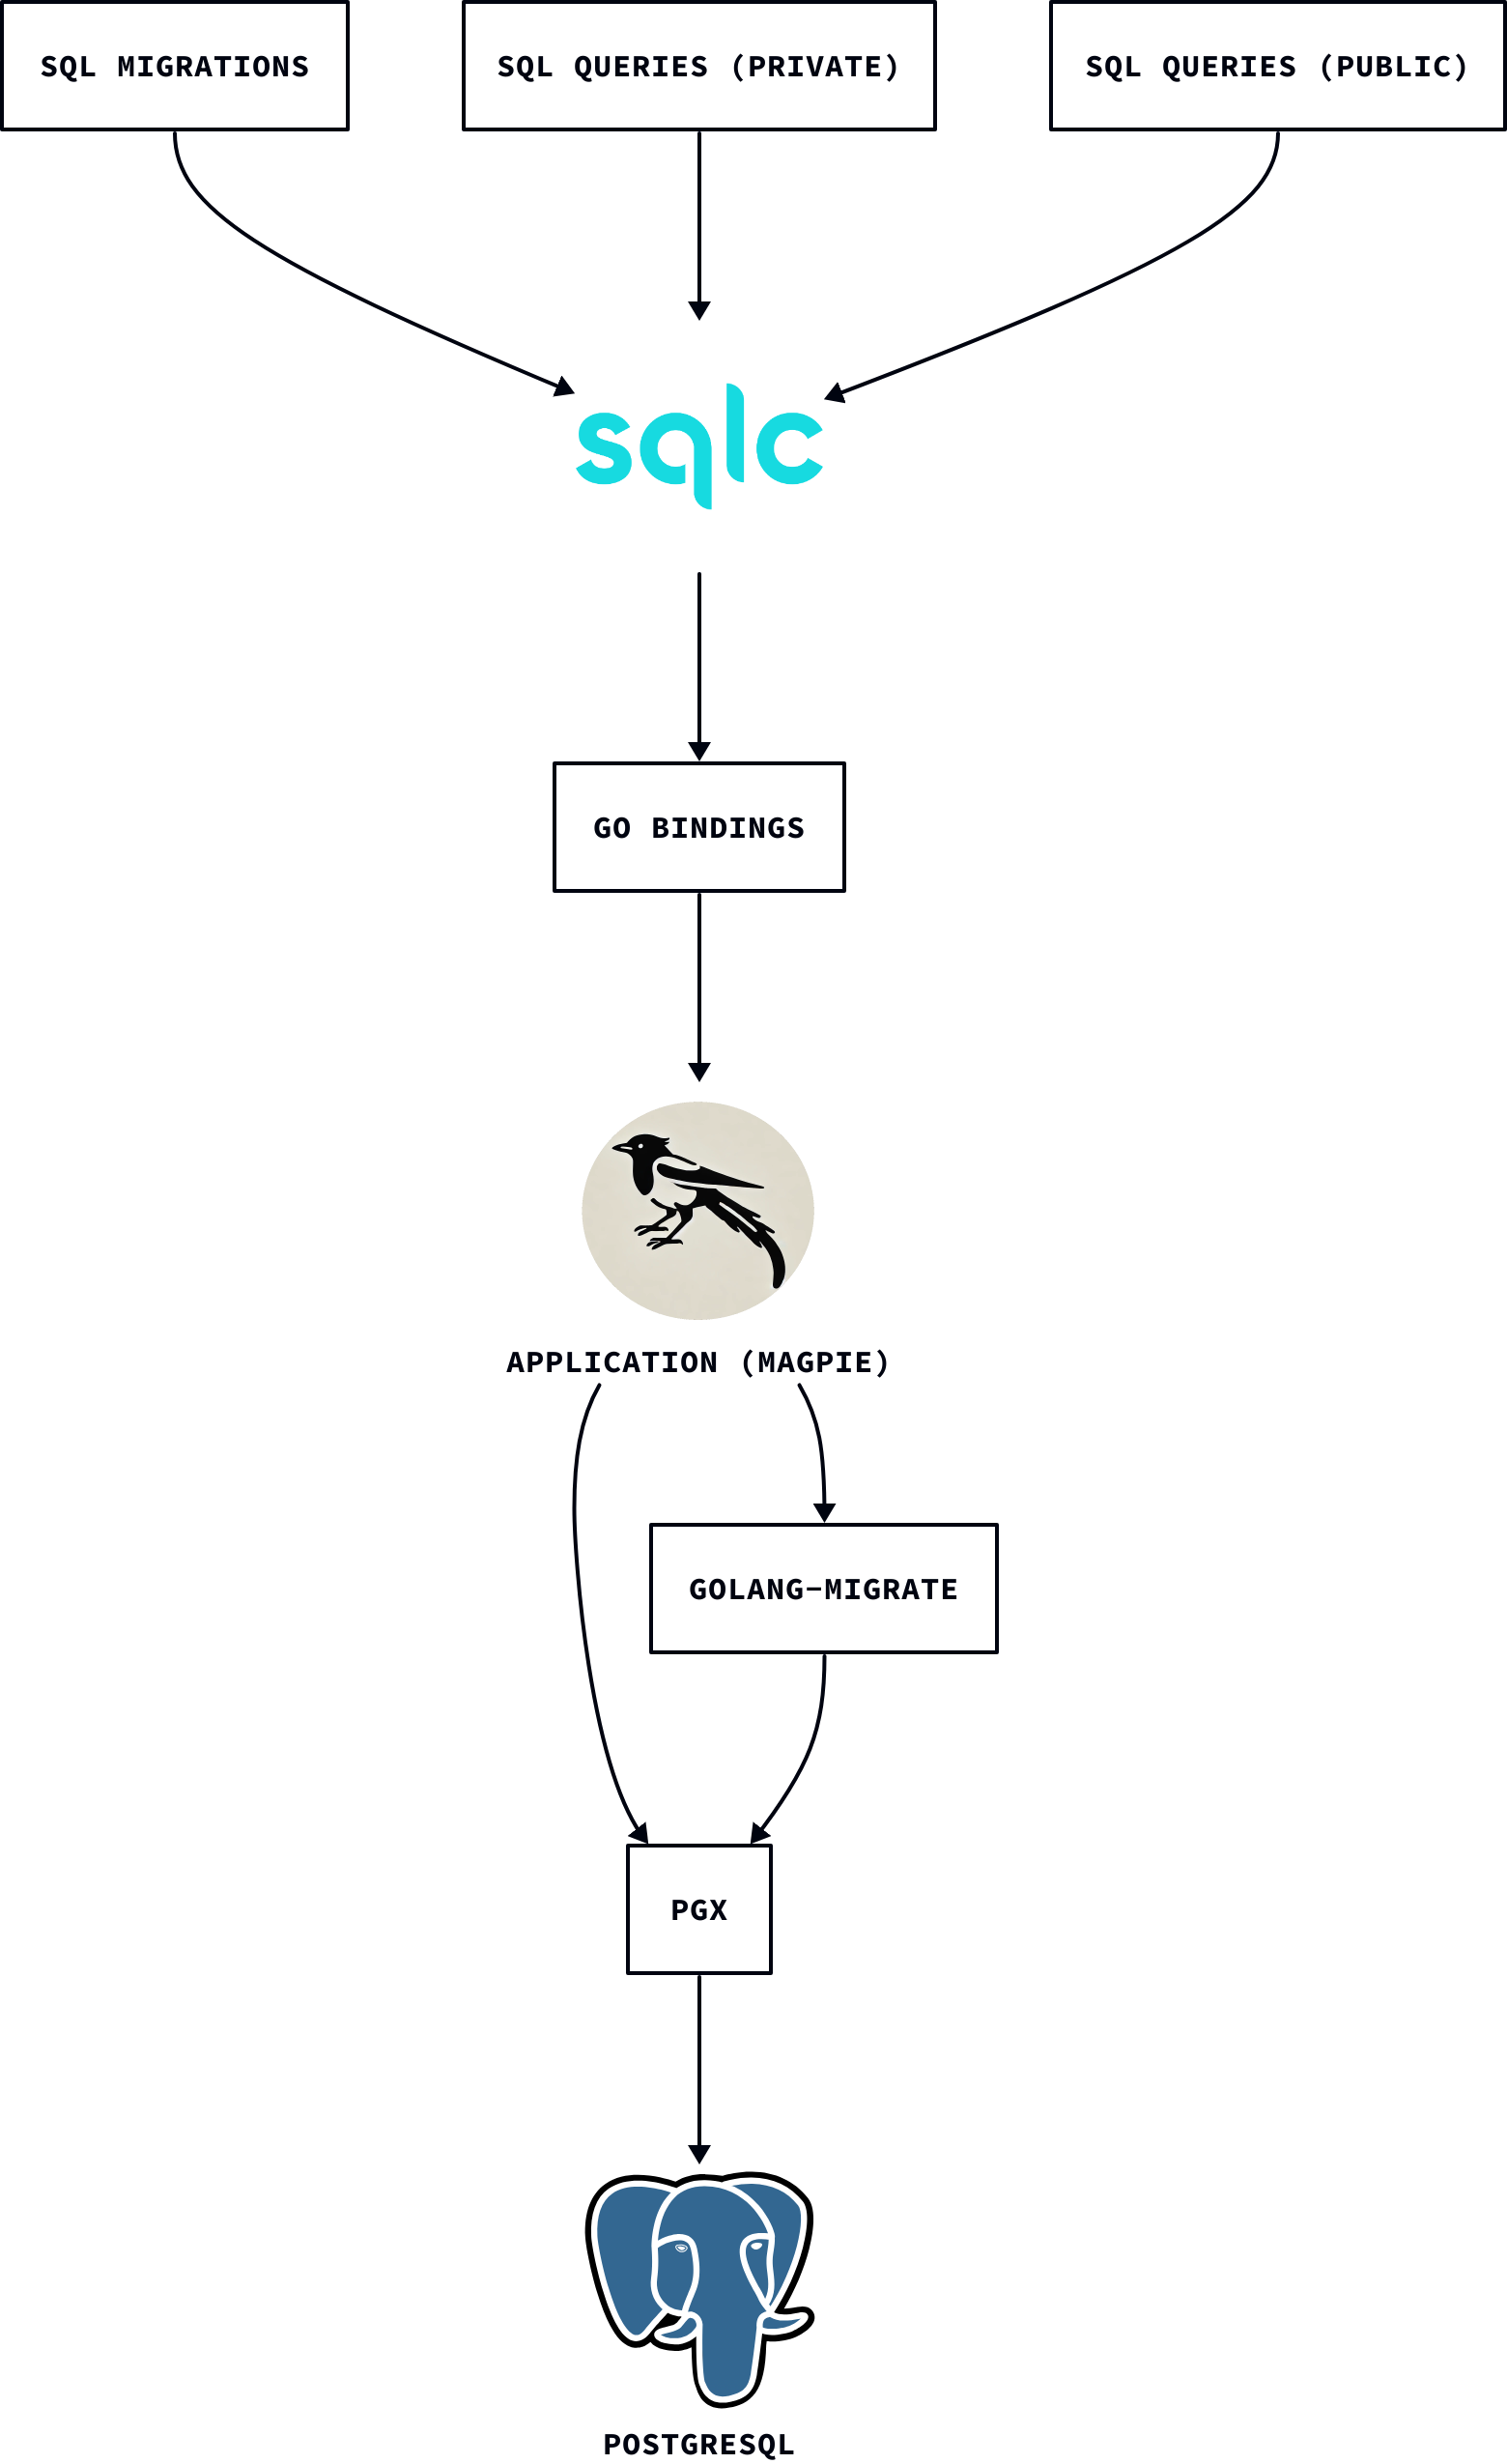
\includegraphics[width=0.8\textwidth]{../d2-diagrams/database-workflow/database_workflow.png}
  \caption{Database Workflow Diagram}
  \label{fig:database_workflow_diagram}
\end{figure}

\paragraph{bcrypt}
To store the users credentials securely, \textbf{bcrypt} was chosen to hash them
before they are inserted into the database. The resulting hashes (see Figure
\ref{fig:bcrypt_hash}) can then be used to validate if the given password is
correct. In accordance with best practices, a work factor of 12 was used when
hashing passwords and a password limit of 72 bytes was implemented
(\cite{owasp_password_storage_cheatsheet}).

While the \textcite{owasp_password_storage_cheatsheet} recommends other, more
recent technologies over bcrypt, they also don't discourage its use in any way.
In the case of Magpie, bcrypt was chosen because the team had past experience
working with it. This was desirable as the registration and login functionality
was deemed to be one of the core features of the MVP. Choosing a technology that
the team did not have any experience could have resulted in slower development,
bugs or even security vulnerabilities as a result of improper implementation.

Since the application was not intended to store highly valuable personal data
such as banking information, personal addresses or health care records it was
deemed acceptable to use a less recent technology in exchange for more rapid
development. Should this project ever evolve into a publicly available and
frequently used application, the use of bcrypt would of course need to be
reevaluated with a much bigger focus on real-world application security rather
than just development speed.

\begin{figure}[H]
  \centering{}
  
\includegraphics[width=0.8\textwidth]{./images/bcrypt_hash.png}
  \caption{Visualisation of a bcrypt hash}
  \label{fig:bcrypt_hash}
\end{figure}

\paragraph{JSON Web Token} \label{jwt}
\textbf{JSON Web Tokens} were chosen for the authentication of user requests to
the APIs. JWTs are JSON objects that are encrypted using a private key on the
server and passed to the frontend when a login requests succeeds. The client is
then expected to pass the token to the backend as a form of authentication in
subsequent requests.

JSON Web Tokens are more than just a simple API token. They can store data about
the authenticated user in them, which can be very useful if the handling of the
requests needs a reference to the user id for example (see example JWT content
in Figure \ref{}). Since the tokens are generated on the backend server using a
private secret, JWTs can be checked for integrity during decoding. Should the
content not match up with the private secret of the backend server, it can be
assumed that the token has been tempered with. In this case, the request would
be discarded and a "Unauthorized" error message would be returned instead.

This structure allows for the authentication system to be decoupled between
backend and frontend. Using JWTs eliminates the need for the backend to keep
track of active sessions, significantly reducing complexity. This and the
familiarity the team had with working with JWTs were ultimately chosen as the
authentication solution for Magpie.

JSON Web Tokens do however come with their own caveats. For example, if any
malicious actor stole such a token from a user, they could pretend to be that
user without the system noticing. JWTs do not have a built-in way to revoke
potentially stolen tokens, neither from the client nor from the server
(\cite{owasp_jwt_cheatsheet}).

Despite these caveats and some slowdowns during development, the team still
feels JWT-based authentication was the right choice for a project of Magpie's
scale.

\subsubsection{Backend Development}
As discussed in \ref{systemarchitecture} \nameref{systemarchitecture}, the
backend is comprised of two standalone REST-API servers. Right after the
decision to split the backend was taken, a first implementation using two
separate codebases was created. This approach was functional, meaning it was
able to produce two distinct backends with different feature sets.

But it soon became obvious that this approach was not sustainable. While simply
splitting the backend into two codebases was a quick and easy solution, it would
almost certainly lead to significantly increased development times in the
future. The two backends have a fair amount of identical functionality and
differ just in the route handlers and the database queries. Leaving the
codebases separate would result in many changes being made twice -- once in the
private backend and once in the public backend.

After careful consideration and discussions with the team, the decision was made
to revert the change that split the backend. The desired result of two distinct
backends would have to be achieved in a different way.

To accomplish this, a feature of the Go programming language called
\textit{build-tags} was utilised. Usage examples of this feature showcase it by
creating multiple binaries that have different feature sets, for instance
multiple different payment tiers for a single software. This was a great
solution for this problem. It allowed for certain files to be excluded during
compilation based on if they were needed for private or public functionality.
While the development of a program split by build-tags is more challenging
than developing a single binary, it is much more streamlined than keeping
functionality identical between two separate projects.

The build-tag system did not fix the problem of code duplication completely
however. Some tools in the Go ecosystem did not handle the exclusive split as
expected. Most notably, the Go language server that provides code completion and
other useful IDE features. It was possible to configure it to recognise files
with their accompanying build-tags, but there was no way to specify exclusivity.
This meant that two files in the same package could not have identical function
definitions even though they would never be included in the binary build process
simultaneously. It was possible to work around this restriction, which it lead
to some code duplication. But this was still a lot better than duplicating the
whole backend.

And while sqlc offers integration for the build-tag system (see the config file
in Listing \ref{listing:sqlc_config_file}), it did not offer to just split the
query part of the generated bindings. As a consequence, the generated code
handling the model bindings and the access to the database had to be generated
and included twice.

\subsubsection{Database}
\fcolorbox{orange}{orange}{Add database development}

\begin{figure}[htbp]
  \centering{}
  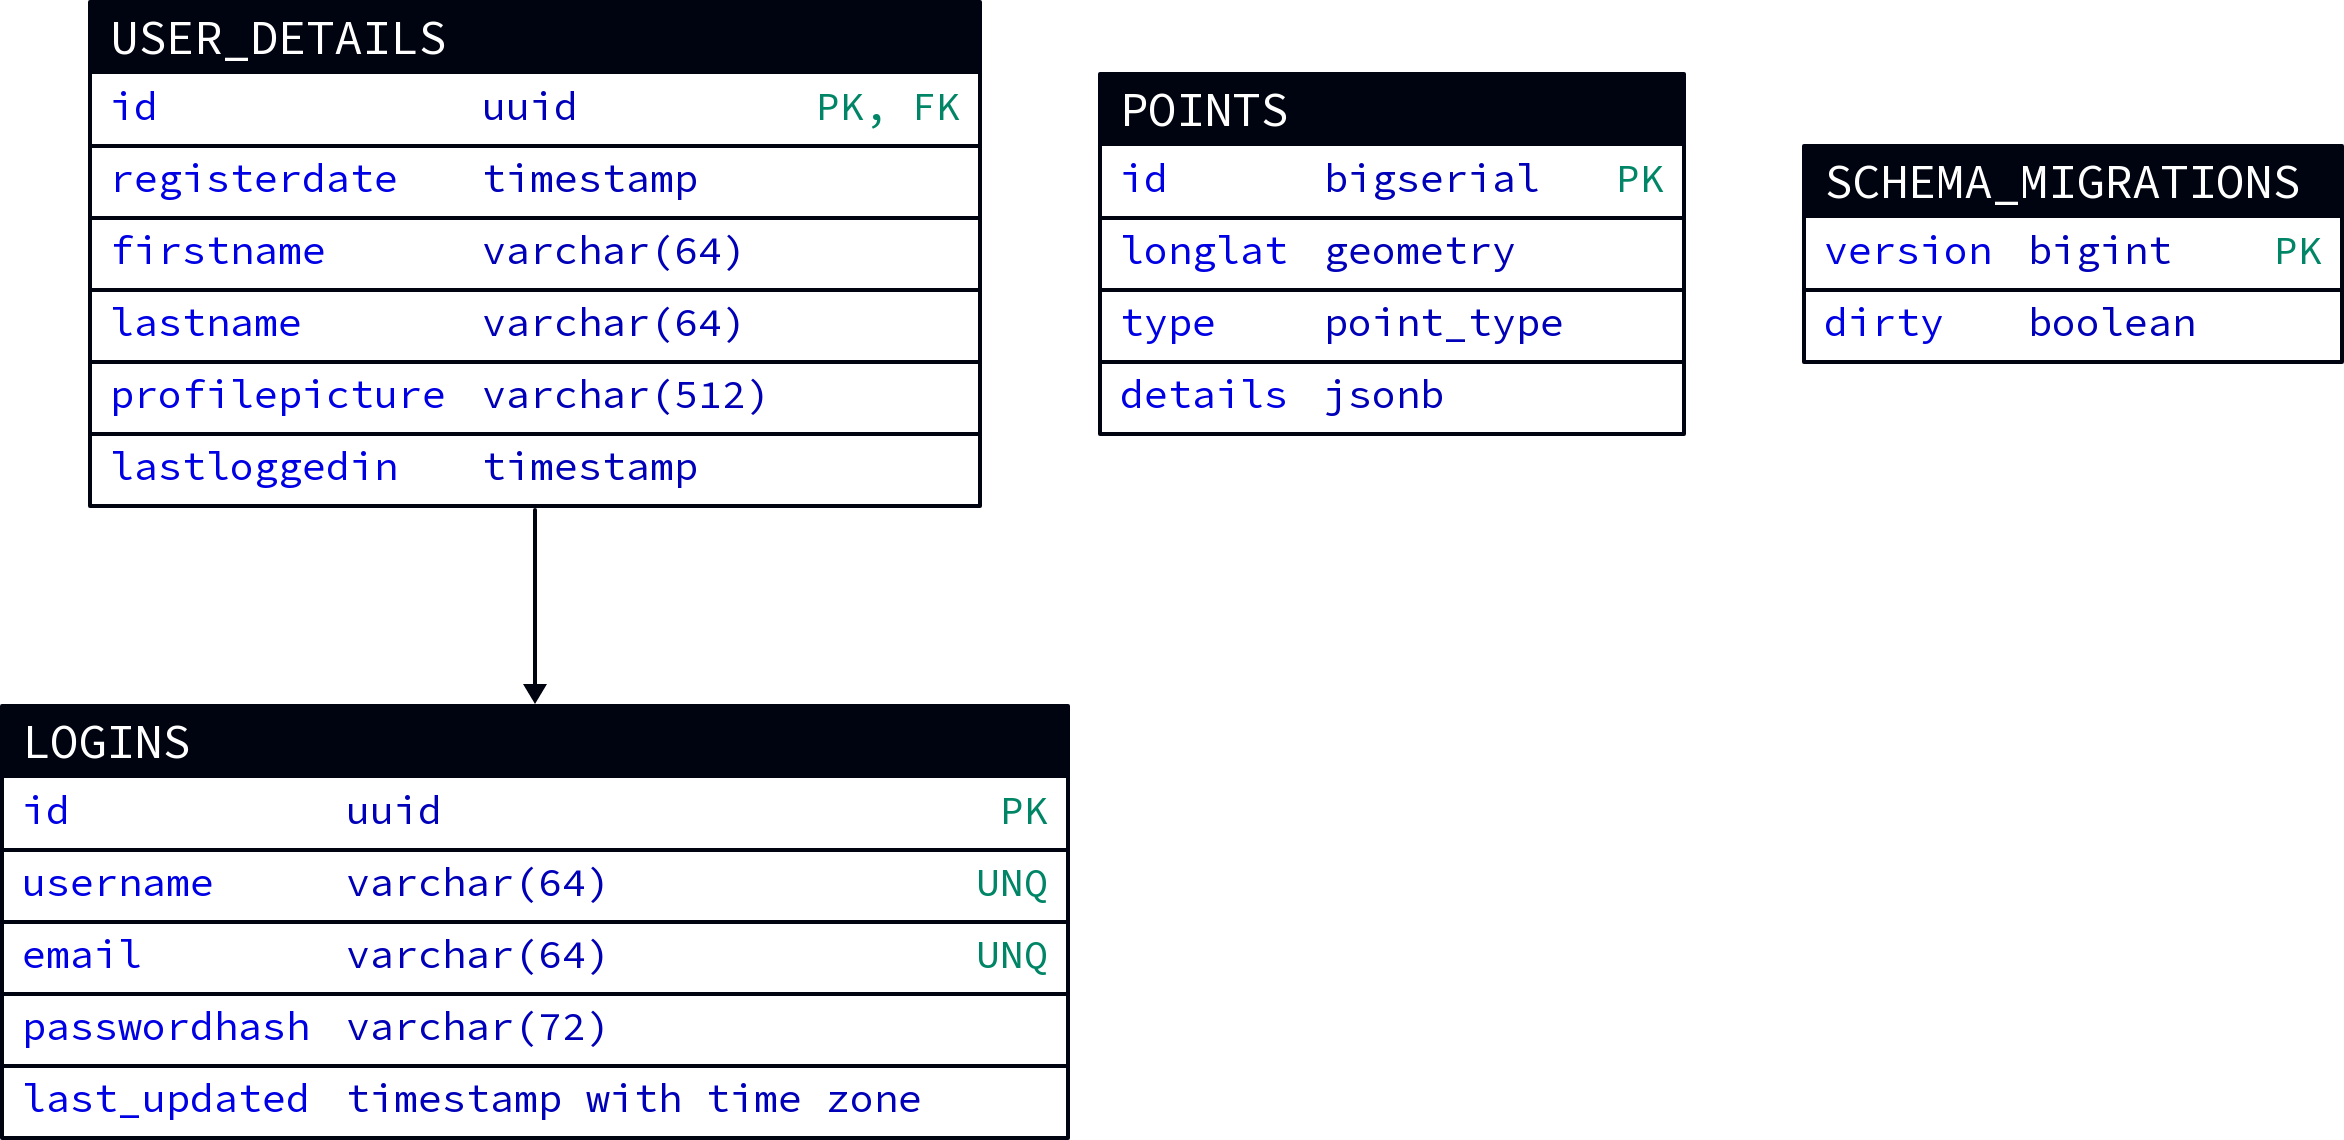
\includegraphics[width=0.8\textwidth]{../d2-diagrams/database-init/database-init.png}
  \caption{Database Schema for the minimum viable Product}
  \label{fig:database_init_schema}
\end{figure}

\begin{figure}[htbp]
  \centering{}
  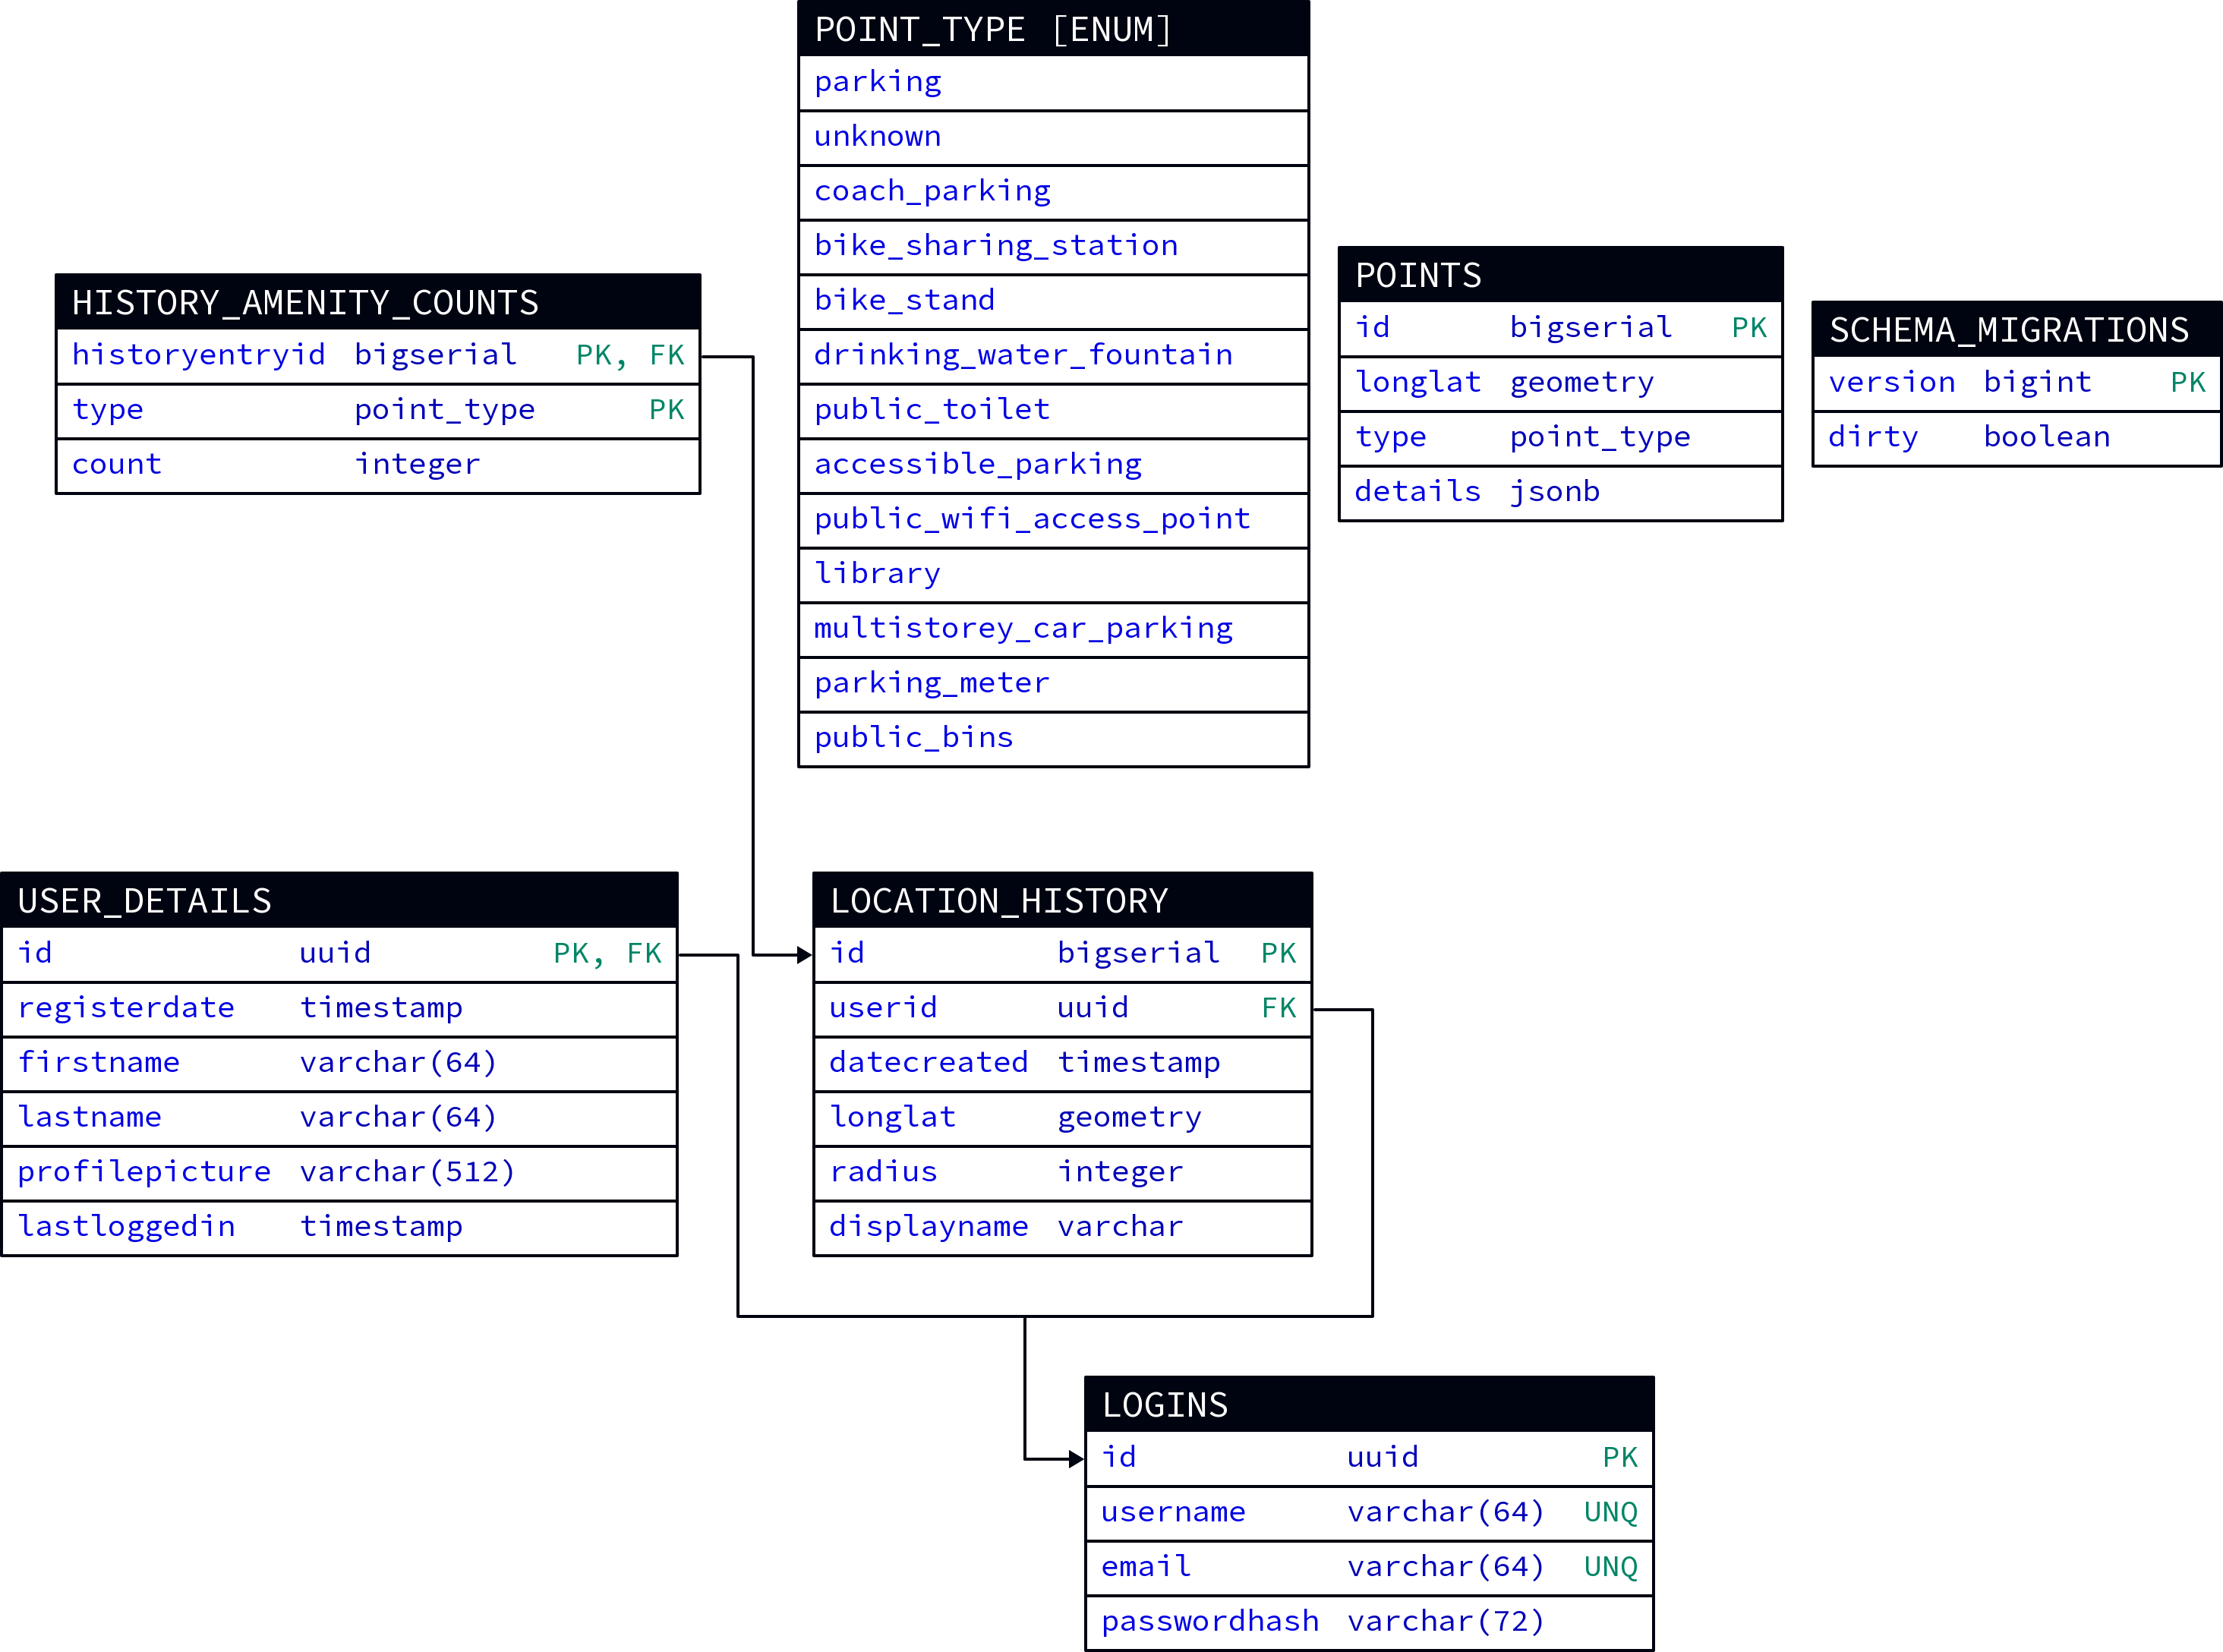
\includegraphics[width=0.8\textwidth]{../d2-diagrams/database-final/database-final.png}
  \caption{Final Database Schema}
  \label{fig:database_final_schema}
\end{figure}

\subsubsection{Routing}
\fcolorbox{orange}{orange}{Add description of net/http library routing}

\subsubsection{APIs}
\paragraph{Public API}
The public API is used by the frontend to retrieve points and authenticate the
user.

\begin{itemize}
  \item{Point Routes
    \begin{itemize}
      \item {\texttt{GET /v1/public/points/\{id\}}}
      \item {\texttt{GET /v1/public/points/inRadius?long=\{\}\&lat=\{\}\&radius=\{\}\&types=\{\}}}
    \end{itemize}
  }
  \item{Saved Location Routes
    \begin{itemize}
      \item {\texttt{GET /v1/public/history/\{id\}}}
      \item {\texttt{DELETE /v1/public/history/\{id\}}}
      \item {\texttt{POST /v1/public/history/\{id\}}}
    \end{itemize}
  }
  \item{Authentication Routes
    \begin{itemize}
      \item {\texttt{POST /v1/public/auth/User/}}
      \item {\texttt{POST /v1/public/auth/User/login}}
      \item {\texttt{GET /v1/public/auth/User/\{id\}}}
      \item {\texttt{PUT /v1/public/auth/User/\{id\}}}
      \item {\texttt{DELETE /v1/public/auth/User/\{id\}}}
    \end{itemize}
  }

  \item {\texttt{GET /heartbeat}}
\end{itemize}

\fcolorbox{orange}{orange}{Add list of public API routes}

\paragraph{Private API}
The private API is used by the machine learning and data stack to insert new
datasets into the database.

\begin{figure}[htbp]
  \centering{}
  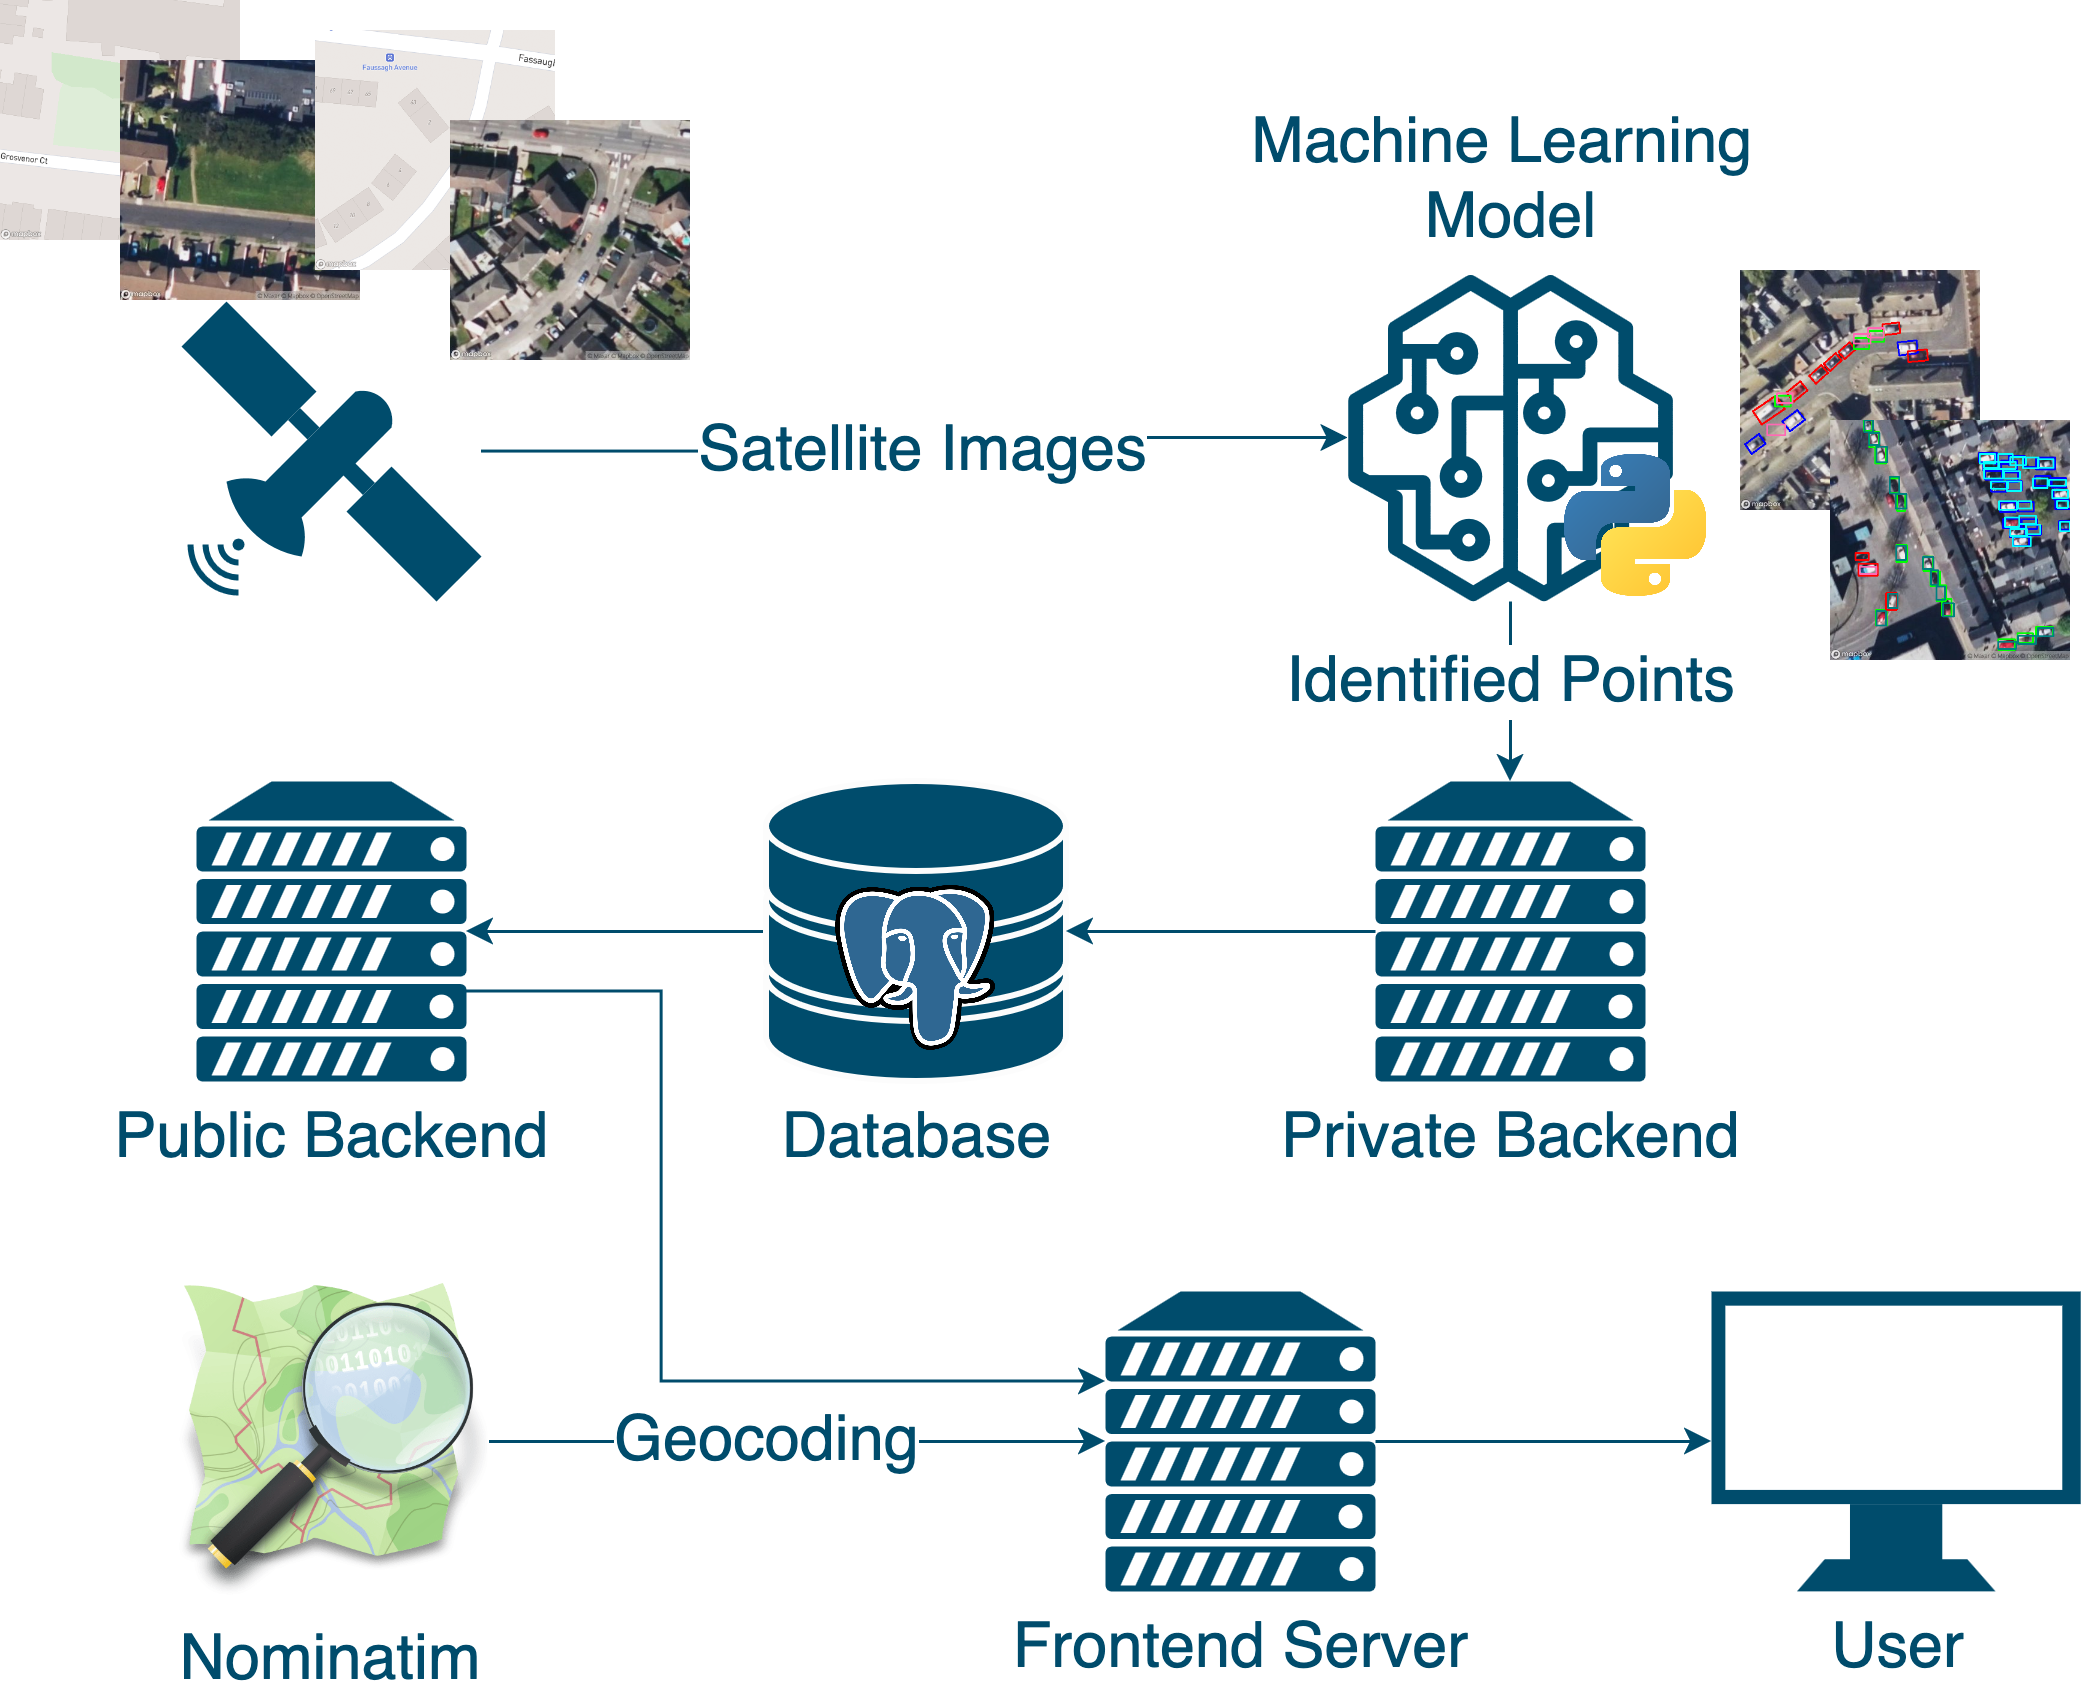
\includegraphics[width=0.8\textwidth]{images/dataflow_5.png}
  \caption{Dataflow Diagram from raw Data to Frontend}
  \label{fig:dataflow}
\end{figure}

\begin{itemize}
  \item {\texttt{POST /v1/private/points}}
  \item {\texttt{PUT /v1/private/points/\{id\}}}
  \item {\texttt{DELETE /v1/private/points/\{id\}}}
  \item {\texttt{GET /heartbeat}}
\end{itemize}

\fcolorbox{orange}{orange}{Add list of private API routes}

\subsubsection{Middlewares}
\paragraph{Authentication}

\fcolorbox{orange}{orange}{Add authentication middleware features}

As mentioned in section \ref{jwt} (\nameref{jwt}), the use of JWTs comes with
its own set of caveats.

One solution for this issue would be implementing a list of revoked tokens on
the server and offering the user a way to add a stolen token to that list. If an
attacker then uses one of these revoked tokens, their requests can be easily
denied. However, this added complexity and development time that the team didn't
have in the MVP phase of the project. So to mitigate the issue, the JWTs were
given a very short expiration time, making them useless after only a few hours.
This led to annoyance and friction during development and testing, so the
expiration time was increased to a week. This made the application less secure,
but much easier to use in both development and regular usage. The backend team
took a unanimous decision to keep the token handling in this state for the time
being, as the application was still considered very much secure enough. The time
and effort needed to implement those additional security features were weighed
up and it became obvious that they would not result in any easily perceptible
improvement to the application.

The issue of improving application security was kept in mind during the whole
development process, but other issues always took precedence. Given more time,
improving the application security would be one of the top priorities in terms
of further backend development.

\paragraph{Authorisation}

\fcolorbox{orange}{orange}{Add route based authorisation}

\subsubsection{Data Validation}
\fcolorbox{orange}{orange}{Add section on data validation}

\subsubsection{Error Handling}
\fcolorbox{orange}{orange}{Add section on error handling}

\subsubsection{Testing}
\fcolorbox{orange}{orange}{Add section on testing}